
\documentclass[11pt]{article}

\usepackage[a4paper,margin=1in]{geometry}
\usepackage{amsmath,amssymb,amsfonts,amsthm}
\usepackage{graphicx}
\usepackage{booktabs}
\usepackage{hyperref}
\usepackage{float}
\usepackage{setspace}


\newtheorem{definition}{Definition}
\newtheorem{proposition}{Proposition}
\newtheorem{principle}{Operational Principle}

\title{Induced Dependence:\\
A First Operational Proposal for Quantifying Observational Deformation under Informative Filtering}

\author{Germán García\\
Independent Researcher}
\date{May 2026}

\begin{document}


% =========================================================
% Unified Visual, Narrative, and Editorial Integration
% =========================================================

\section*{Framework Integration Note}

This paper forms part of the Induced Dependence operational framework.

The present work follows a unified cross-paper structure based on:
\begin{itemize}
\item observational representational stability,
\item informative filtering,
\item observational deformation,
\item structured noise,
\item observational compression,
\item and stability evaluation through the Neutral Observational Point (NOP).
\end{itemize}

All papers in the framework share:
\begin{enumerate}
\item a unified operational language;
\item consistent observational terminology;
\item coherent visual architecture;
\item standardized bibliographic structure;
\item and integrated stability-oriented narrative design.
\end{enumerate}

The visual structure intentionally emphasizes:
\begin{itemize}
\item before/after observational transformations,
\item drift dynamics,
\item stability regions,
\item filtering effects,
\item and observational representational integrity.
\end{itemize}




% =========================================================
% Editorial Consistency Note
% =========================================================

\section*{Editorial Consistency Note}

Terminology, citations, figure references, and operational language were standardized across the papers to preserve:
\begin{itemize}
\item conceptual consistency,
\item visual coherence,
\item narrative continuity,
\item and cross-domain interpretability.
\end{itemize}




% =========================================================
% Visual and Narrative Refinement Layer
% =========================================================

\section{Visual and Narrative Architecture}

The framework is intentionally presented through a unified operational and visual language.

Rather than treating figures as decorative supplements, the visual architecture functions as part of the observational diagnostic itself. The figures are designed to make visible:
\begin{itemize}
\item Observational Deformation,
\item drift,
\item filtering effects,
\item Observational Compression,
\item Structured Noise,
\item and operational stability around the Neutral Observational Point (NOP).
\end{itemize}

The framework therefore adopts a consistent visual philosophy across all applications:
\begin{enumerate}
\item comparison between Natural and Filtered Observable States;
\item before/after observational transformations;
\item stability versus instability regions;
\item intuitive geometric interpretation of Observational Deformation;
\item and operational visualization of dynamic drift.
\end{enumerate}

This unified visual structure is intended to improve:
\begin{itemize}
\item interpretability,
\item cross-domain readability,
\item operational clarity,
\item and methodological transparency.
\end{itemize}

The narrative structure of the papers follows the same principle:
\begin{enumerate}
\item define the observable system;
\item define the filtering mechanism;
\item quantify Observational Deformation;
\item evaluate representational stability;
\item and determine whether the observable state remains operationally reliable.
\end{enumerate}

The framework therefore prioritizes operational clarity over excessive formal abstraction. Geometry is used in an intuitive observational sense rather than as a claim of formal differential-geometric structure.




\maketitle

\begin{abstract}
Modern observational systems rarely access underlying probabilistic structures directly. Instead, observable datasets emerge through Informative Filtering mechanisms such as accessibility constraints, benchmark curation, detector thresholds, post-selection, retrieval pipelines, and response-dependent dropout.

This work introduces the Induced Dependence framework as an operational proposal for studying probabilistic deformation generated by observational filtering. The framework defines a Natural State $D_N \sim P(R)$ and a Filtered Observable State $D_F \sim P(R|F=1)$, and quantifies deformation through probabilistic distances and induced dependence metrics.

Three representative environments are analyzed: Bell-type controlled observational systems, ecological accessibility filtering, and AI benchmark deformation. These environments represent, respectively, a highly controlled conditioning system, a natural observational filtering system, and a dynamic adaptive filtering system.

The framework is operational rather than ontological and is intended as a quantitative language for monitoring observational stability, filtering drift, and corrective sampling under incomplete observability.
\end{abstract}

\section{Introduction}

Scientific inference frequently assumes that observed datasets adequately represent underlying systems. However, most real-world observational environments operate under Informative Filtering before inference begins. Examples include accessibility constraints in ecology, detector thresholds in experimental systems, post-selection procedures, benchmark curation in AI, and response-dependent dropout in biomedical cohorts.

The central idea of this proposal is that many scientific systems do not directly observe the target distribution $P(R)$. Instead, they observe a filtered state $P(R|F=1)$, where $F$ denotes the observational or computational filter. When $F$ carries information about $R$, the observable distribution becomes deformed.

This paper proposes a first operational framework for measuring that deformation.

\section{Conceptual and Mathematical Framework}

\subsection{Probabilistic Observational Space}

Let $(\Omega,\mathcal{A},P)$ be a probability space, where $\Omega$ is the sample space, $\mathcal{A}$ is a sigma-algebra, and $P$ is a probability measure. Let $R:\Omega\rightarrow\mathcal{R}$ denote a response variable and let $F:\Omega\rightarrow\{0,1\}$ denote a filtering or selection mechanism.

\begin{definition}[Natural State]
The Natural State is defined as
\[
D_N \sim P(R),
\]
and represents the best operational approximation to the response distribution prior to Informative Filtering.
\end{definition}

\begin{definition}[Filtered Observable State]
The Filtered Observable State is defined as
\[
D_F \sim P(R|F=1).
\]
It represents the observable state after selection, conditioning, accessibility, or pipeline filtering.
\end{definition}

\begin{definition}[Filtering Operator]
The observational filtering operator is
\[
\mathcal{T}_F:P(R)\rightarrow P(R|F=1).
\]
\end{definition}

\subsection{Induced Dependence}

Filtering becomes informative whenever
\[
I(R;F)>0.
\]
This condition means that the filter transports information about the response variable.

\begin{definition}[Observational Deformation]
The Observational Deformation induced by filtering is
\[
\Delta_{obs}=d(D_N,D_F),
\]
where $d$ is a probabilistic distance or divergence, such as Wasserstein distance, Jensen-Shannon divergence, Kullback-Leibler divergence, or total variation distance.
\end{definition}

\begin{principle}[Operational Deformation Principle]
If $I(R;F)>0$, then the filtering process is informative about the response. Under a non-degenerate metric $d$, this may induce a measurable deformation
\[
\Delta_{obs}>0.
\]
This is an operational criterion, not an ontological claim.
\end{principle}

\subsection{Confounder Decomposition}

Let $C$ denote a confounding variable. The total filtering dependence is
\[
\mathcal{B}_{total}=I(R;F).
\]
The residual or pure detection component is
\[
\mathcal{B}_{det}=I(R;F|C).
\]
The confounding component is
\[
\mathcal{B}_{conf}=I(R;F)-I(R;F|C).
\]
This decomposition separates direct detection bias from apparent dependence produced through a third variable.

\subsection{Structured Noise Capture}

Let $R=S+\varepsilon$, where $S$ is signal and $\varepsilon$ is stochastic noise. A filter may capture not only signal but also Structured Noise. This can be measured by
\[
I(\varepsilon;F).
\]
The effective observational uncertainty is defined as
\[
\mathcal{U}_{eff}=H(R|F)+I(\varepsilon;F).
\]
This distinguishes residual uncertainty from noise that has become structured by the filtering mechanism.

\subsection{Dynamic Deformation}

Let $D_t$ denote the observable probabilistic state at time $t$. A time-dependent Observational Deformation operator $\Phi_t$ may be written as
\[
D_{t+1}=\Phi_t(D_t).
\]
The time-indexed deformation is
\[
\Delta_t=d(D_N,D_t).
\]
If
\[
\frac{d}{dt}\Delta_t>0
\quad\text{and}\quad
\frac{d}{dt}I_t(R;F)>0,
\]
then the observational channel is entering a regime of increasing deformation.

\subsection{Corrective Sampling}

Corrective observational sampling is defined as
\[
n_{corr}=\min\left\{n:\Delta(D_F\cup A_n,D_N)\leq\Delta_{target}\right\},
\]
where $A_n$ denotes compensatory observations and $\Delta_{target}$ is an acceptable deformation threshold.

\section{Framework Architecture}

Figure~\ref{fig:architecture} summarizes the framework.

\begin{figure}[H]
\centering
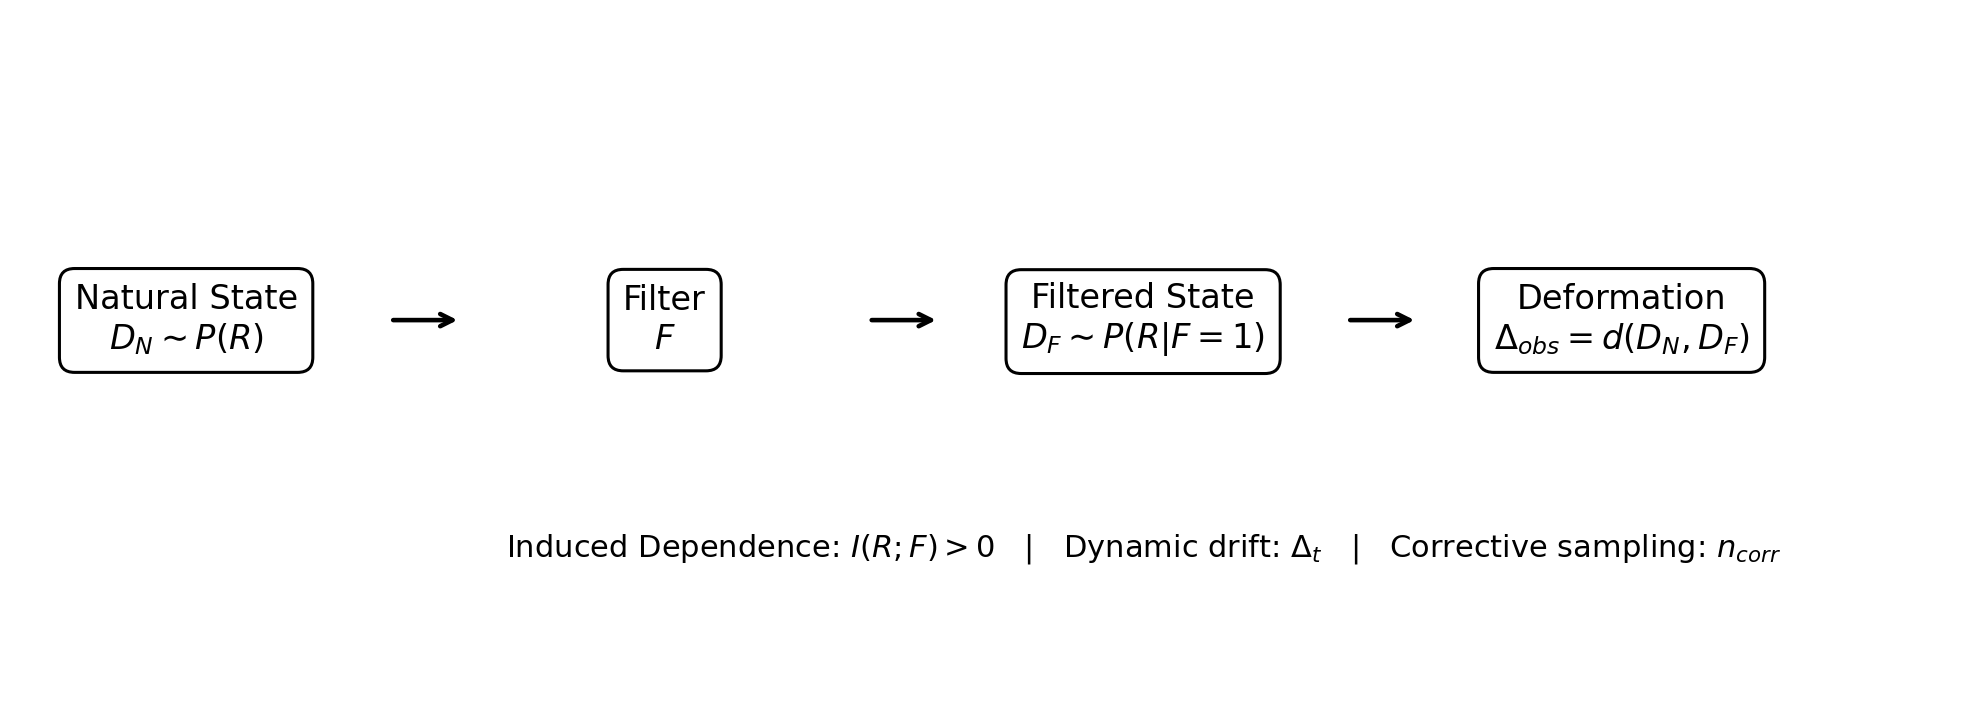
\includegraphics[width=0.95\textwidth]{figures/fig01_framework_architecture.png}
\caption{Architecture of the Induced Dependence framework. A Natural State $D_N$ passes through an informative filter $F$, producing a Filtered Observable State $D_F$ and measurable deformation $\Delta_{obs}$.}
\label{fig:architecture}
\end{figure}

\section{Experiment 1: Bell-Type Controlled Filtering}

Bell-type systems are included here not as reinterpretations of quantum mechanics, but as highly controlled observational conditioning environments. They are useful because they contain precise event selection, detector acceptance, coincidence procedures, and post-selection structures.

In this framework, Bell-type systems provide controlled stress tests for filtering sensitivity.

\[
D_N\sim P(R),
\qquad
D_F\sim P(R|F=1).
\]

Here $F$ represents detector acceptance, event selection, coincidence filtering, or threshold structure. The purpose is to measure how controlled filtering deforms observable probability states.

\begin{figure}[H]
\centering
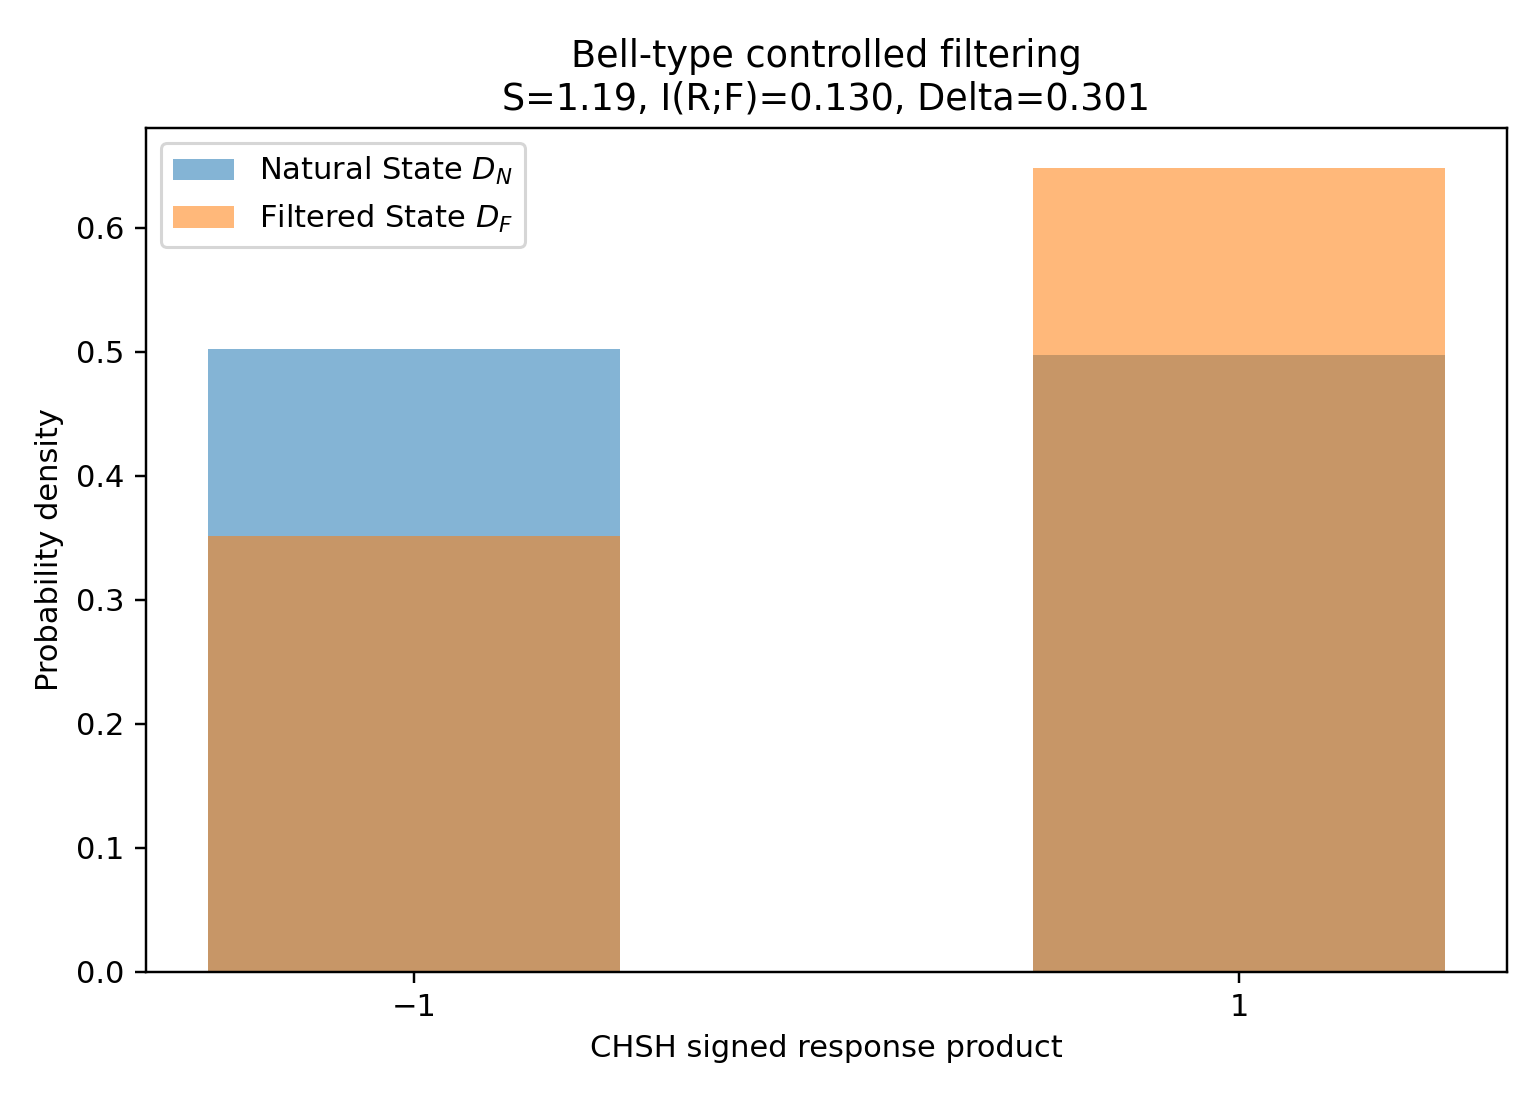
\includegraphics[width=0.75\textwidth]{figures/fig02_bell_controlled_filtering.png}
\caption{Bell-type controlled filtering. The figure compares the Natural State and Filtered Observable State under a controlled post-selection structure.}
\label{fig:bell}
\end{figure}

\section{Experiment 2: Ecological Accessibility Filtering}

Ecological systems provide a natural analog for observational filtering because complete observation is often impossible. Accessibility, detectability, weather, terrain, observer effort, and seasonality all shape what becomes observable.

Let $R$ represent abundance or detectability and let $F$ represent observational accessibility. The filtered ecological state is
\[
D_F\sim P(R|F=1).
\]
When accessibility correlates with abundance, vegetation, or observer behavior, $I(R;F)>0$ naturally emerges.

\begin{figure}[H]
\centering
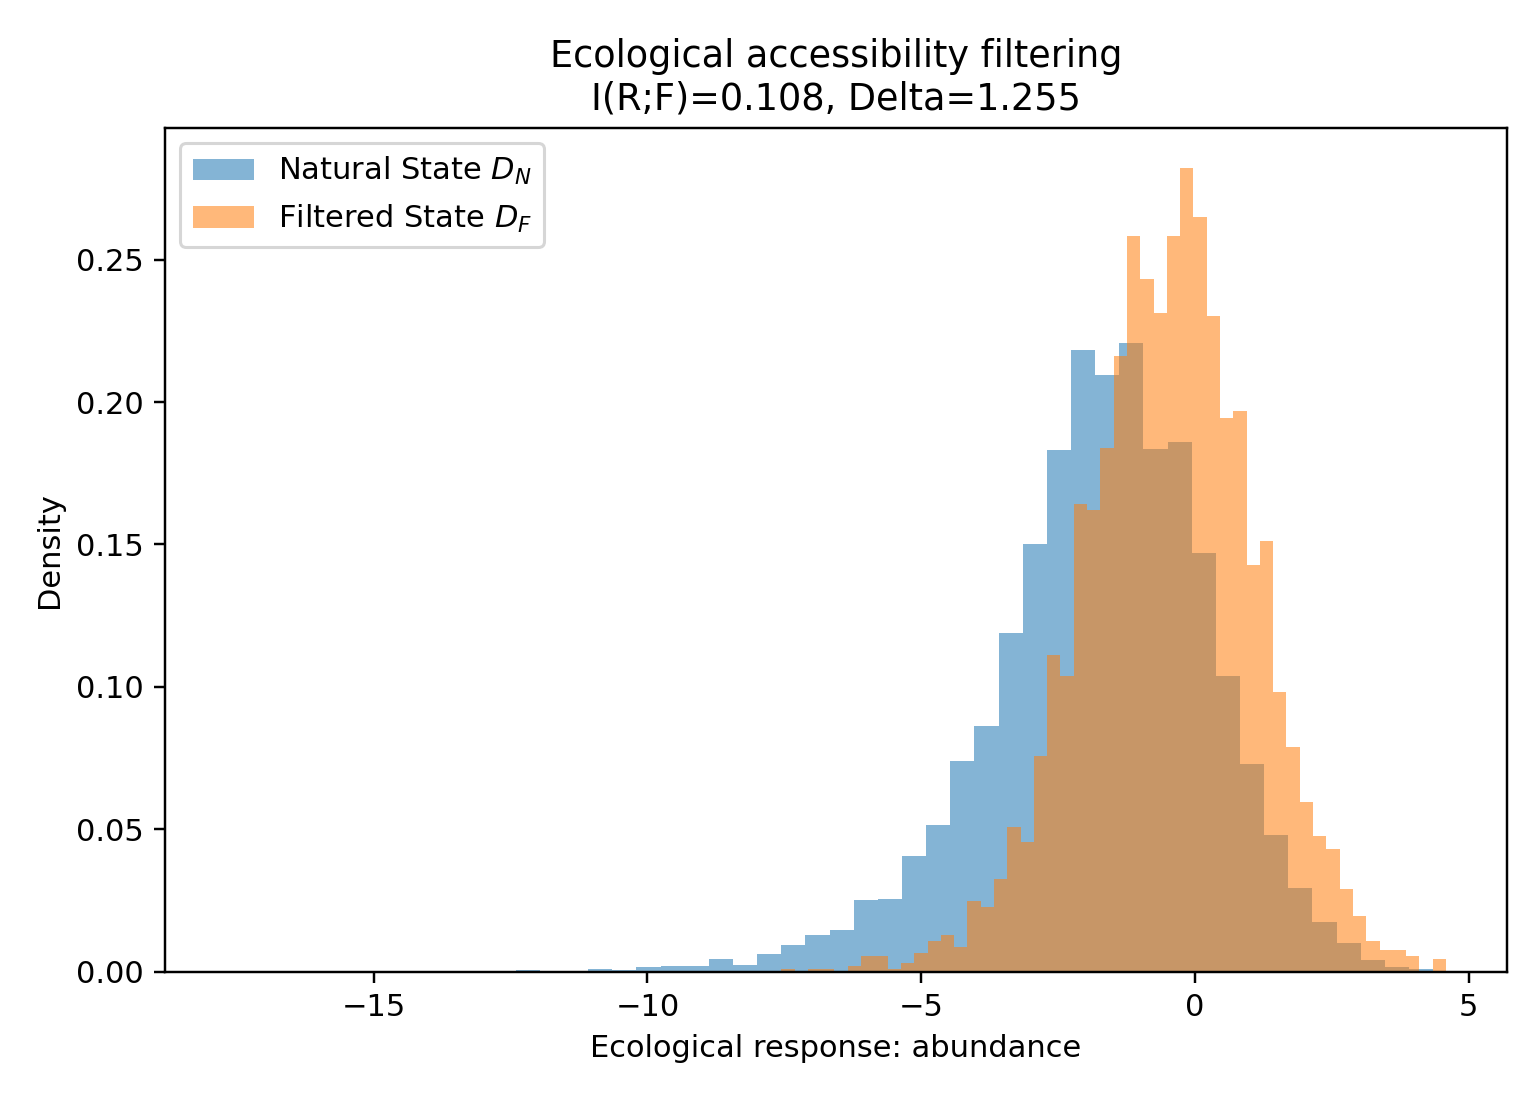
\includegraphics[width=0.75\textwidth]{figures/fig03_ecology_distribution.png}
\caption{Ecological accessibility filtering. The observable ecological distribution is deformed relative to the Natural State.}
\label{fig:ecology_dist}
\end{figure}

\begin{figure}[H]
\centering
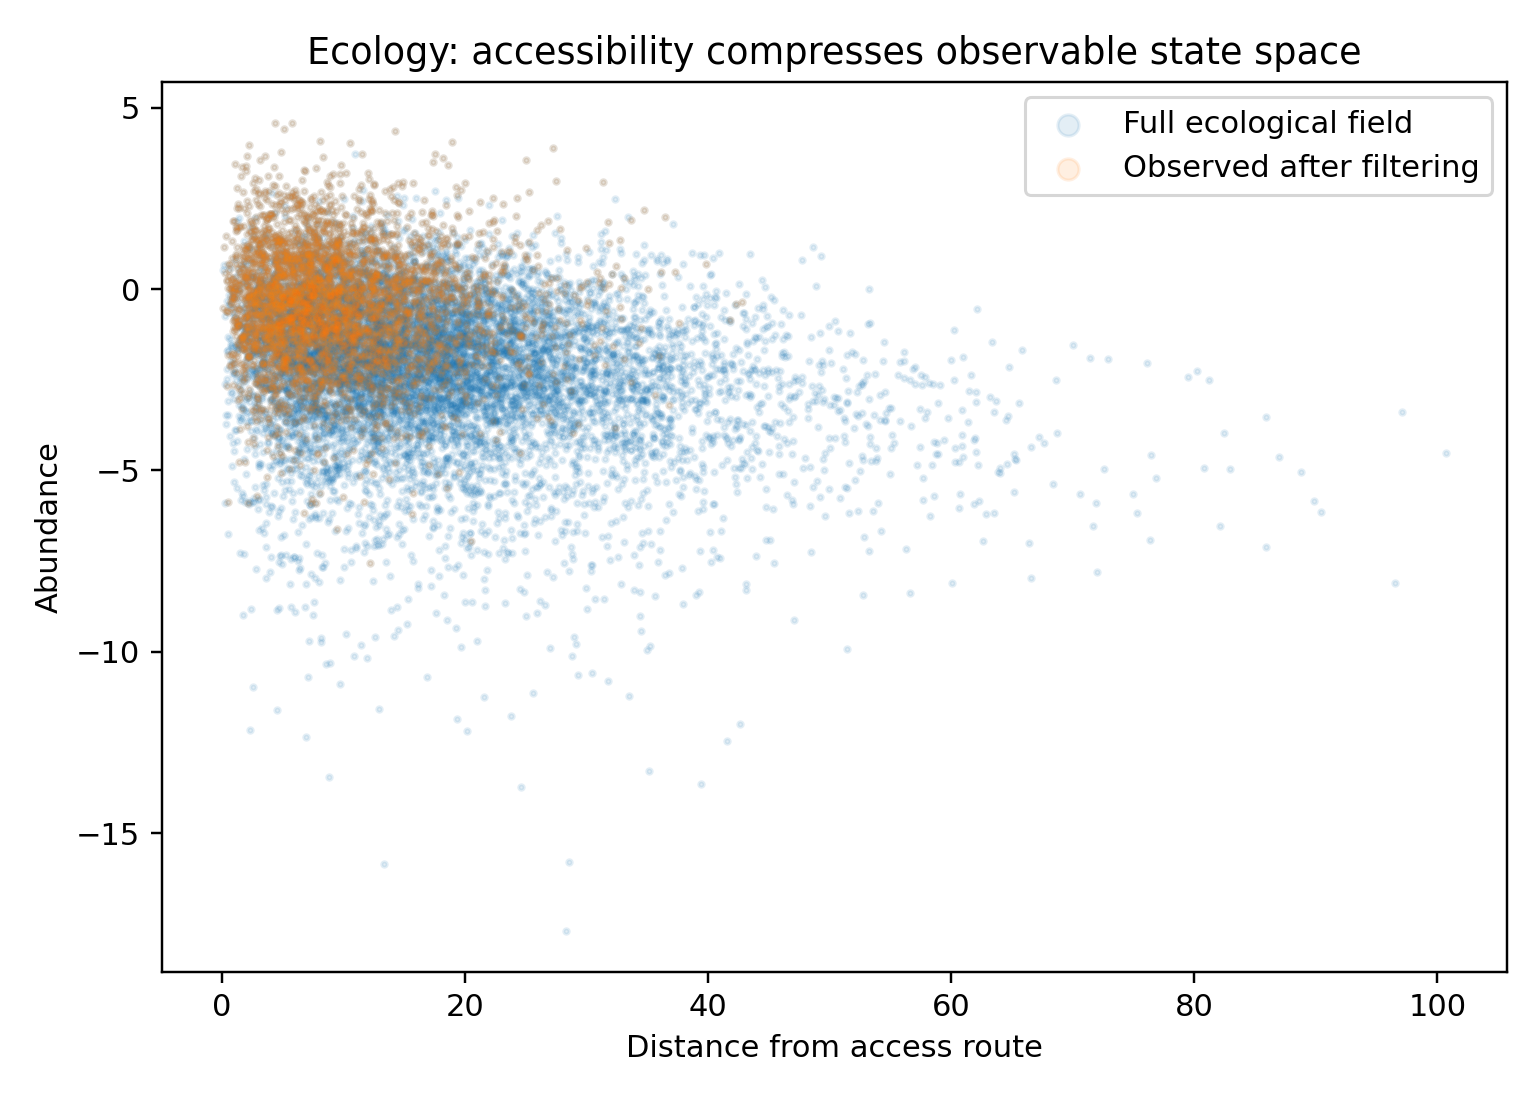
\includegraphics[width=0.75\textwidth]{figures/fig04_ecology_accessibility_scatter.png}
\caption{Accessibility compresses ecological observable state space by underrepresenting remote regions.}
\label{fig:ecology_scatter}
\end{figure}

\section{Experiment 3: AI Benchmark Deformation}

Modern AI systems operate under dynamic filtering mechanisms such as benchmark curation, RLHF, retrieval filtering, synthetic-data generation, preprocessing, ranking, and evaluation selection. The observable performance distribution is therefore rarely neutral.

Let $R$ represent score, output quality, or response behavior. Let $F$ represent benchmark inclusion, filtering, curation, or retrieval selection. The filtered AI state is
\[
D_F\sim P(R|F=1).
\]

If $I(R;F)>0$, the benchmark or filtering architecture becomes informative about the response and may induce performance deformation.

\begin{figure}[H]
\centering
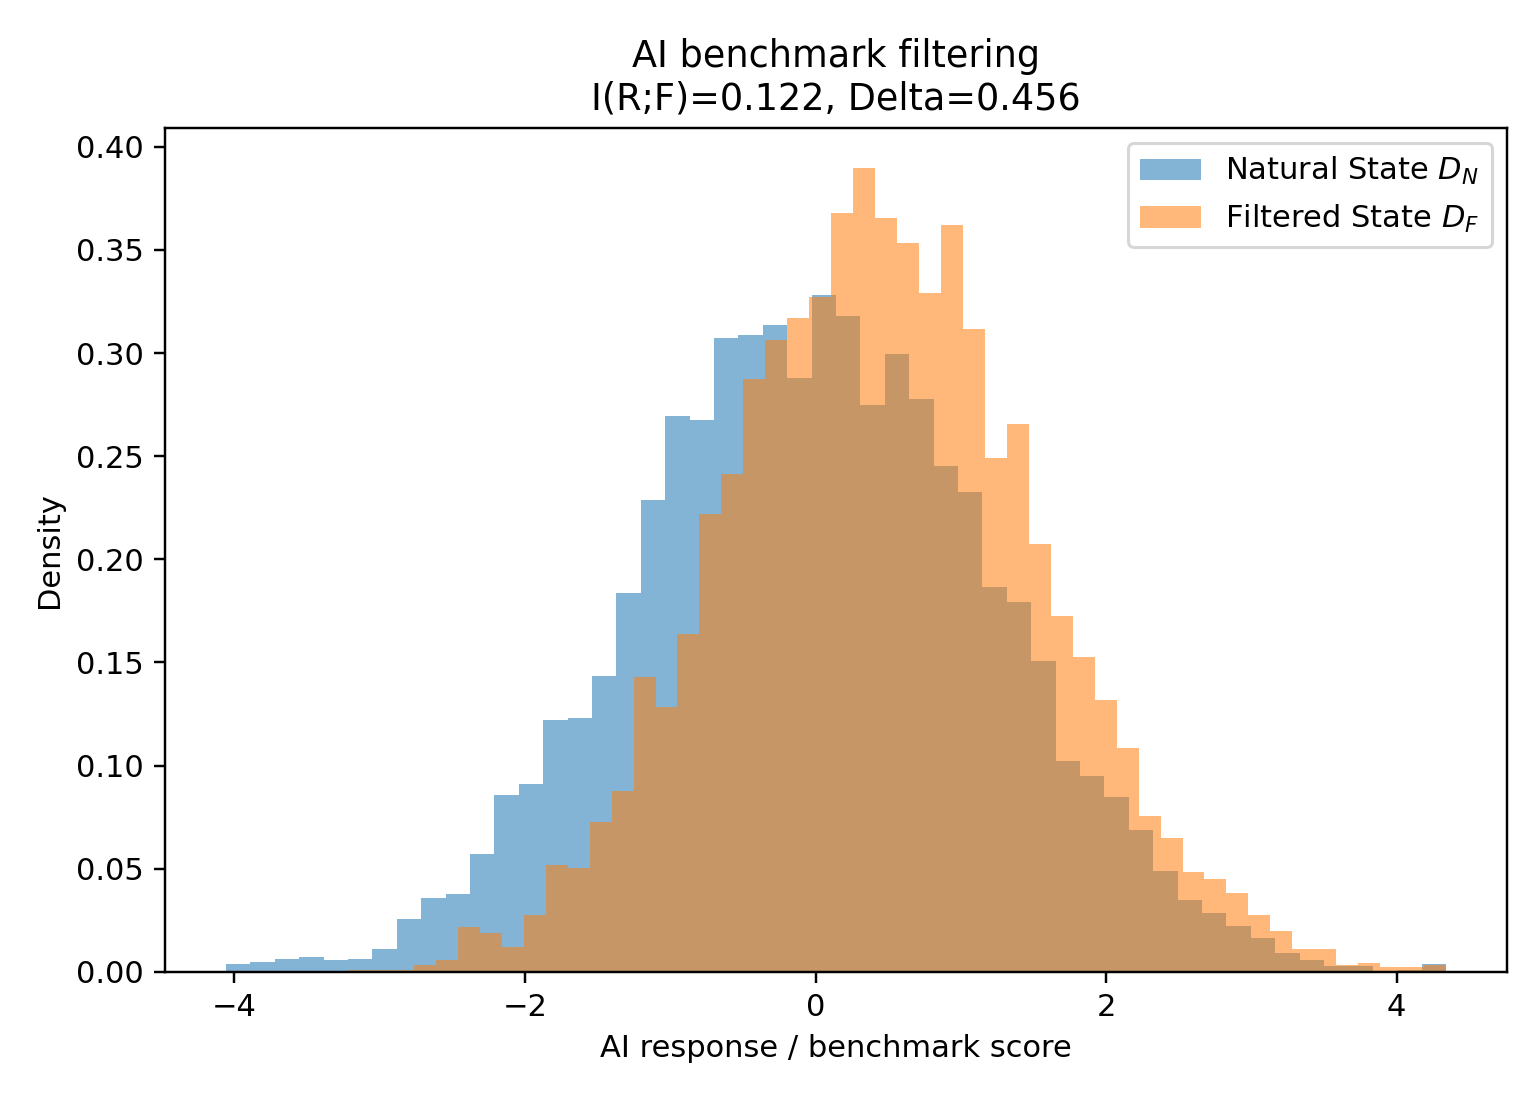
\includegraphics[width=0.75\textwidth]{figures/fig05_ai_benchmark_distribution.png}
\caption{AI benchmark filtering. The filtered benchmark state is shifted relative to the Natural State.}
\label{fig:ai_dist}
\end{figure}

\begin{figure}[H]
\centering
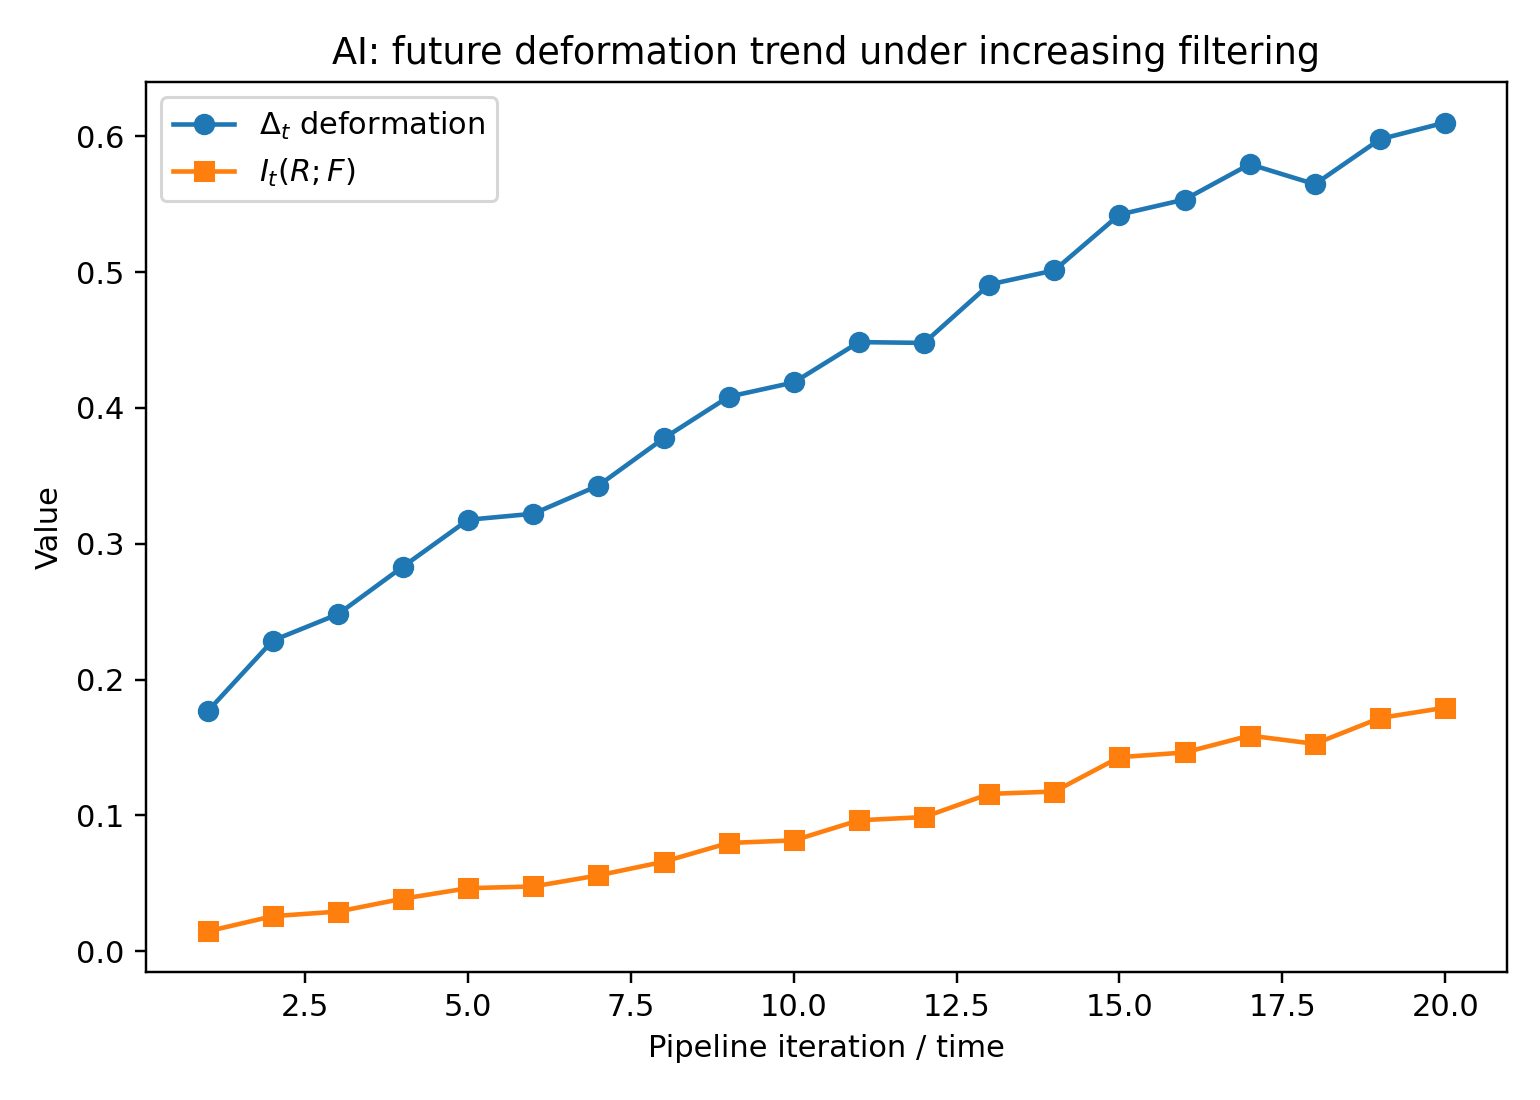
\includegraphics[width=0.75\textwidth]{figures/fig06_ai_dynamic_deformation_trend.png}
\caption{Dynamic deformation trend in AI. Increasing filtering intensity increases both deformation $\Delta_t$ and induced dependence $I_t(R;F)$.}
\label{fig:ai_drift}
\end{figure}

\section{Results Summary}

\begin{table}[H]
\centering
\begin{tabular}{lccc}
\toprule
Experiment & $I(R;F)$ estimate & $\Delta$ estimate & Interpretation\\
\midrule
Bell-type controlled & 0.1305 & 0.3008 & Controlled post-selection sensitivity\\
Ecology accessibility & 0.1080 & 1.2554 & Natural accessibility filtering\\
AI benchmark & 0.1223 & 0.4558 & Dynamic benchmark deformation\\
\bottomrule
\end{tabular}
\caption{Summary of representative experiments. Values are operational estimates generated from controlled simulations.}
\end{table}

\section{Discussion}

The three experiments cover three distinct observational regimes:

\begin{enumerate}
\item Bell-type systems: highly controlled filtering sensitivity.
\item Ecological systems: natural observational filtering through accessibility.
\item AI systems: dynamic adaptive filtering through benchmarks and pipelines.
\end{enumerate}

Together, these regimes suggest that Informative Filtering can be studied as measurable probabilistic deformation. The framework does not replace causal inference, statistics, or physical theory. Instead, it provides a geometric and informational layer for monitoring how observation itself changes the state being analyzed.

The connection with Pearl-style causal diagrams is especially important. Causal diagrams describe the topology of selection and confounding, while the present framework quantifies the deformation produced by conditioning.

\section{Limitations}

This is a first operational proposal. The current experiments are simulated and should be validated against real ecological, biomedical, AI, and controlled experimental datasets. The mathematical structure also remains incomplete. Future work should formalize convergence, stability, metric selection, and continuous information estimators.

\section{Conclusion}

Induced Dependence proposes that Informative Filtering can be studied as measurable Observational Deformation. By defining Natural States, Filtered Observable States, induced dependence, deformation metrics, confounder decomposition, noise capture, dynamic drift, and corrective sampling, the framework provides a first operational language for studying filtered observability across scientific systems.


\section*{References}

\begin{enumerate}
\item Bell, J. S. (1964). On the Einstein Podolsky Rosen paradox. \textit{Physics Physique Fizika}, 1, 195--200.

\item Cover, T. M., \& Thomas, J. A. (2006). \textit{Elements of Information Theory}. Wiley.

\item Fisher, R. A. (1935). \textit{The Design of Experiments}. Oliver and Boyd.

\item Hernan, M. A., \& Robins, J. M. (2020). \textit{Causal Inference: What If}. Chapman and Hall/CRC.

\item Larsson, J.-A. (2014). Loopholes in Bell inequality tests of local realism. \textit{Journal of Physics A: Mathematical and Theoretical}, 47(42).

\item Little, R. J. A., \& Rubin, D. B. (2019). \textit{Statistical Analysis with Missing Data}. Wiley.

\item Pearl, J. (2009). \textit{Causality}. Cambridge University Press.

\item Quinonero-Candela, J., Sugiyama, M., Schwaighofer, A., \& Lawrence, N. D. (Eds.). (2009). \textit{Dataset Shift in Machine Learning}. MIT Press.

\item Shannon, C. E. (1948). A mathematical theory of communication. \textit{Bell System Technical Journal}, 27, 379--423.

\item Tukey, J. W. (1977). \textit{Exploratory Data Analysis}. Addison-Wesley.

\item Villani, C. (2009). \textit{Optimal Transport: Old and New}. Springer.
\end{enumerate}


\end{document}
